%====================================================================================================
% En-tête
%====================================================================================================
\begin{figure}[H]
    \centering
    \includegraphics[scale=0.65]{assets/figures/Mechanical Design/Système.png}
    \caption{Representation of the Mechanical design}
    \label{fig:Mec_Blobal}
\end{figure}
\newpage
%====================================================================================================
% Preliminary choices and limitations
%====================================================================================================
\section{Preliminary choices and limitations}
\subsection{Objectives}
First, the mechanical system need to be attached to the output of the laboratory telescope. To achieve this, an adaptor piece is
required (\ref{sec:adaptator}). Then, the masks will need to be attached to a support (\ref{sec:mask}). A second support will have
to be made to accommodate the prisms (\ref{sec:prisms}). Finally, the lens must be installed (\ref{sec:lens}) and the camera placed
just behind it (\ref{sec:Camera}). \newline
The system must be compact, adjustable and adaptable if modifications are required at a later date.
\subsection{Limitations}
To make this system a reality, a simple and common fastening system had to be integrated. The most simple system used in optical design 
is the cage system. Two of the world's leading optomechanics manufacturers offer it (Thorlabs and Edmund Optics). The significant difference 
between these 2 manufacturers is the spacing between the steel bars. This difference is shown in the capter \ref{sec:lens}. \newline
To integrate the telescope's occular correctly, the Edmund optics system is required. This is because the distance between the steel bars 
is smaller on the thorlabs system, and the distance between the occular and the bore for the bar would be far too small ($\approx$ 0.05mm).
\bigbreak
The difference between the Thorlabs system and the Edmund Optics system is the centering diameters for the steel bar holes who 
can be seen on the figure \ref{fig:thorlabs_Edmund} ($\emptyset\ 38\ mm$ for Thorlabs (blue) and $\emptyset\ 57\ mm$ for Edmund optics (red))
\begin{figure}[H]
    \centering
    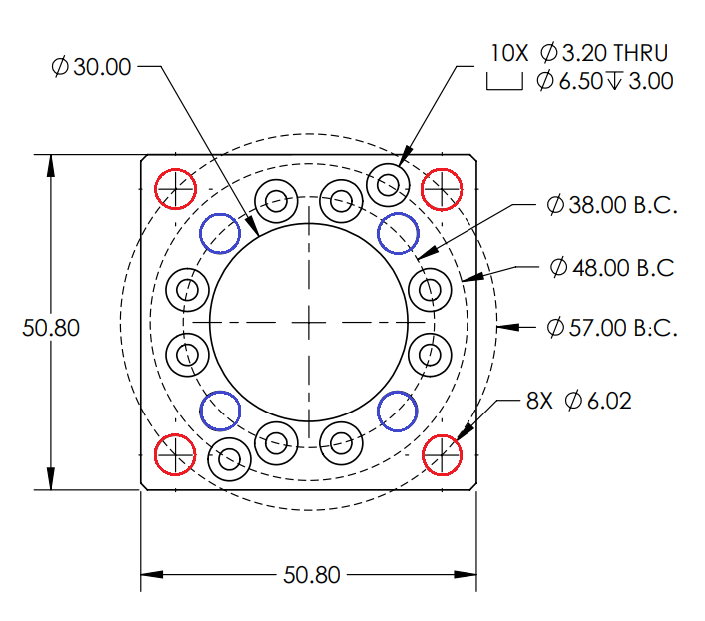
\includegraphics[scale=1]{assets/figures/Mechanical Design/Thorlabs_Edmund.png}
    \caption{Differences between thorlabs and Edmund systems}
    \label{fig:thorlabs_Edmund}
\end{figure}
%====================================================================================================
% Telescope mounting system
%====================================================================================================
\section{Telescope mounting system}\label{sec:adaptator}
The telescope-mounting system, as its name suggests, will be the connecting piece between the telescope output and the DIMM. It will 
also integrate the telescope's occular. The choice of integrating the telescope's ocular with this part was made to improve the system's 
stability and alignment. The system will be screwed onto the telescope, so it won't be held in place by simple screws attached to 
the part. \newline
This part will maintain all the DIMM. So it need to be strong and more massive than the other parts. However, it also needs to be as 
light as possible so as not to weigh too much on the telescope. Material was therefore removed from the middle of the piece to reduce 
its weight.
\bigbreak
Figure \ref{fig:Mec_Adapter1} (Adapter drawing) shows :
\begin{enumerate}
    \item The hole for the ocular ($\emptyset\ 33.55\ mm$) and the thread for its attachment ($MF\ 40\ P=1$). Fixing is simply done 
    with a threaded ring drilled through the center.
    \item The thread for attaching the system to the telescope ($\emptyset\ 50.75\ mm\ TPI\ 24$)
    \item Hole for steel bars and the screws used to secure them ($\emptyset\ 6.02$)
\end{enumerate}
\begin{figure}[H]
    \centering
    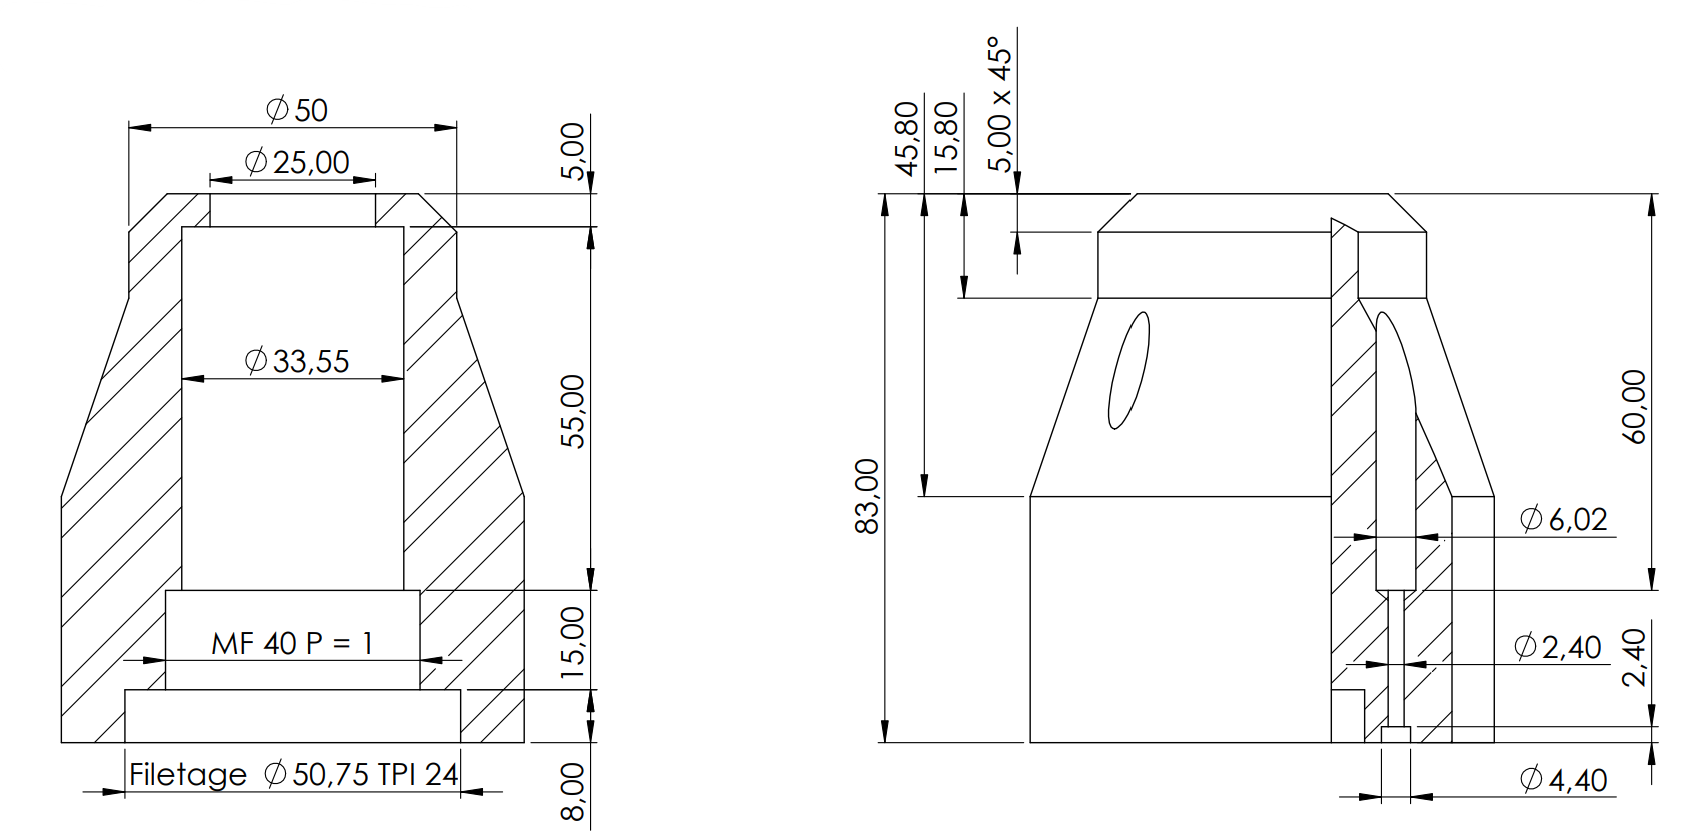
\includegraphics[scale=0.6]{assets/figures/Mechanical Design/Dessin_Part1_adapter.png}
    \caption{Representation of the adaptator : ocular and bar fixation}
    \label{fig:Mec_Adapter1}
\end{figure}
This part will be made of aluminum to reduce its weight. The use of aluminum has no effect on the rigidity of the system. \newline
However, the ocular attachment ring will be made of steel to limit the coefficient of friction when screwing it on 
(screwing an aluminum part with another of this material will have a grip effect between the two parts).
\bigbreak
The complete drawing can be found in the appendix \ref{App:MEP}
\newpage
%====================================================================================================
% Mask mounting
%====================================================================================================
\section{Mask and mounting}\label{sec:mask}
\subsection{Mask}
As explained in section \ref{sec:Opti_Limit}, the mask will have 2 holes 1mm in diameter, with their centers 5mm apart. 
A 0.5mm-thick plate was designed for this purpose. This plate includes the 2 holes and is shaped to fit more easily into its support.
This part is shown in figure \ref{fig:Mec_Mask}
\begin{figure}[H]
    \centering
    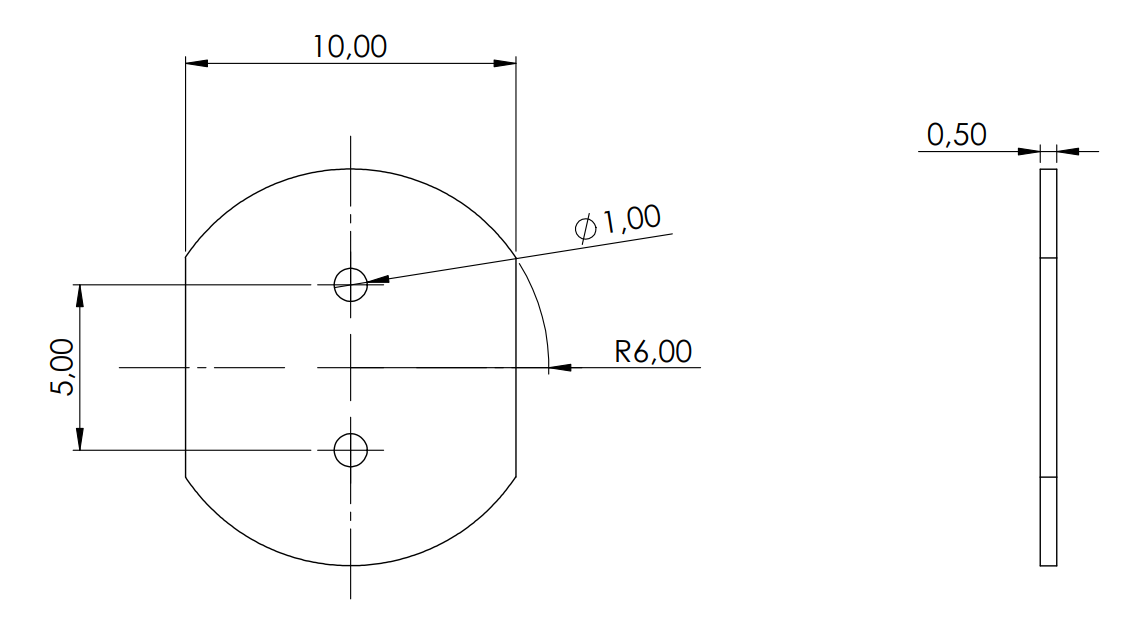
\includegraphics[scale=0.55]{assets/figures/Mechanical Design/Dessin_Mask.png}
    \caption{Drawing of the mask}
    \label{fig:Mec_Mask}
\end{figure}
\subsection{Mounting}
For the support, 2 pieces are required. The first will contain the "rail" where the mask will be inserted (Figure \ref{fig:Mec_Mask_Sup_Rail} left),
 and the other will hold it in place (Figure \ref{fig:Mec_Mask_Sup_Rail} right).
\begin{figure}[H]
    \centering
    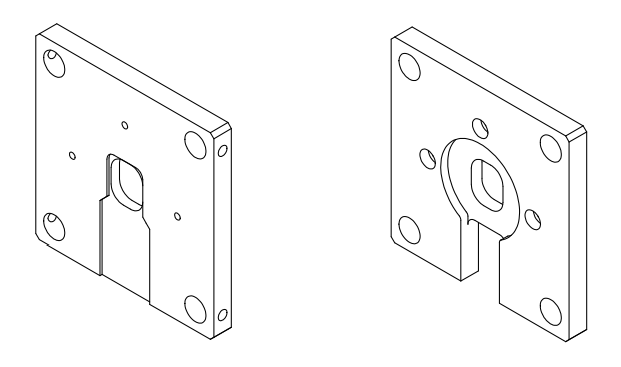
\includegraphics[scale=0.85]{assets/figures/Mechanical Design/Support_masque_rail.png}
    \caption{Supports for the mask}
    \label{fig:Mec_Mask_Sup_Rail}
\end{figure}
Figure \ref{fig:Mec_Mask_Sup_Rail} (left) shows the mask positioning rail, the tapped holes for attaching the second part and the holes 
for the steel bars. \newline
Figure \ref{fig:Mec_Mask_Sup_Rail} (right) shows the second piece who is designed for easy mask removal. This part also features the opening 
for inserting the mask, as well as the screw holes for securing the two parts together.\bigbreak
This part will be made of aluminum to reduce its weight. The use of aluminum has no effect on the rigidity of the system.
\bigbreak
The complete drawing can be found in the appendix \ref{App:MEP}
%====================================================================================================
% Prisms and mounting
%====================================================================================================
\section{Prisms and mounting}\label{sec:prisms}
\subsection{Prisms}
As explained in section 2, the output beams from the prism must have an angle of incidence of 1°. 
This corresponds to an angle of 1.93° on the prism. \newline
Several requests for bids were made, but none were within the budget allocated under the TB. The aim was to have a square-shaped 
prism (\ref{fig:Prism_square} left) to reduce the size of the system and make it easier to assemble. However, this solution could not be retained and the 
use of circular prisms (\ref{fig:Prism_square} right) was required. This solution greatly reduces the budget, but the part that will hold them will be much more complex.
\begin{figure}[H]
    \centering
    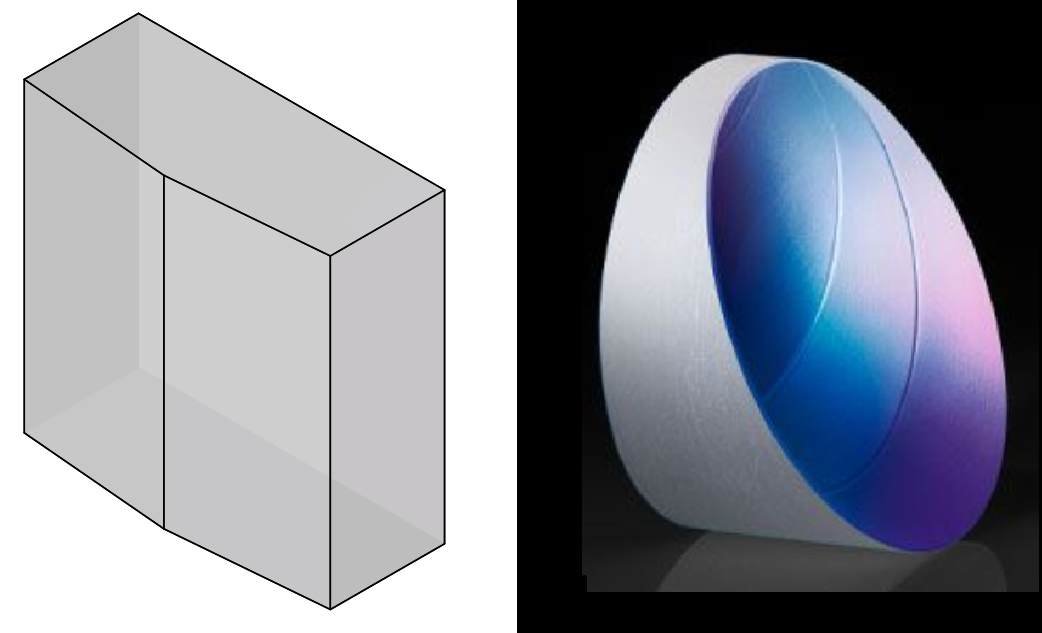
\includegraphics[scale=0.5]{assets/figures/Mechanical Design/prisme_voulu.png}
    \caption{Needed prism / Prism choosed}
    \label{fig:Prism_square}
\end{figure}
\subsection{Mounting}
To attach the 2 prisms, we had to create a custom-made part. To achieve this, several elements were critical 
like direction, position and orientation of the prism.
\bigbreak
For these purpose, a maintenance part has been created (Figure \ref{fig:Prism_Support1}). This part will allow the 2 prisms to be inserted, while letting 
the beam from the mask pass through. \newline
There are 2 small notches on the back of the part. These notches are there to ensure correct mounting of the prism's 
holding parts (Figure \ref{fig:Prism_Support2}).\newline
This part also has holes and threads for fixing the assembly to the steel bars, and for attaching the part that 
will hold the prisms in position. 
\begin{figure}[H]
    \centering
    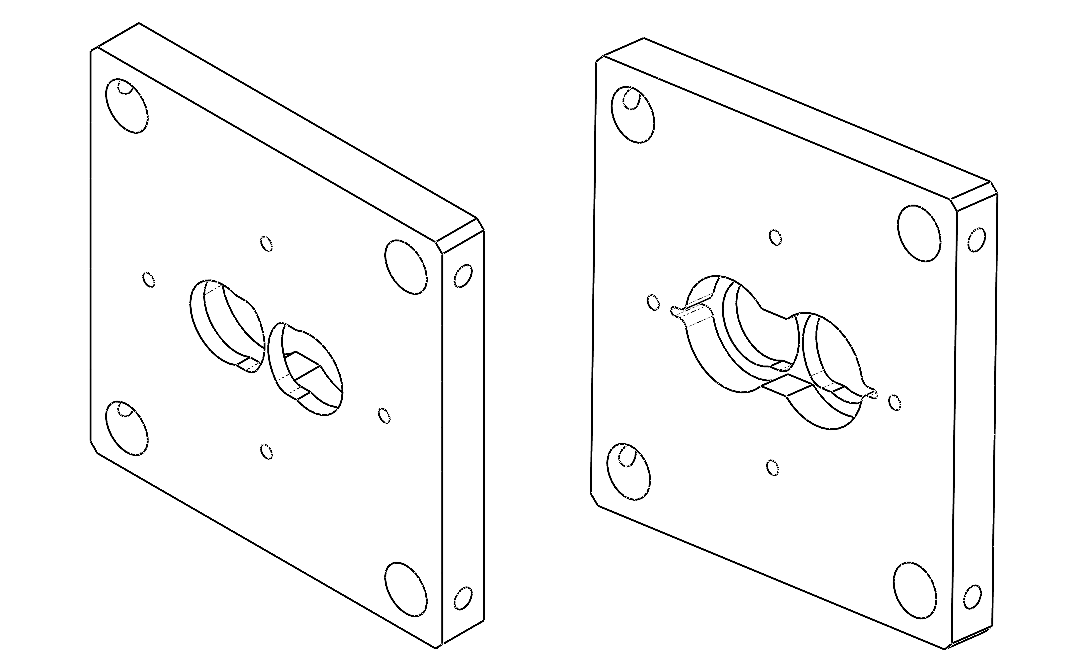
\includegraphics[scale=0.55]{assets/figures/Mechanical Design/MaintientPrism1.png}
    \caption{Support for the prisms}
    \label{fig:Prism_Support1}
\end{figure}
The part shown in figure \ref{fig:Prism_Support2} was created to fix and hold the prisms correctly. This part fits perfectly into the support 
bore and will be positioned with the notches. \newline 
This part is made with the same angle of inclination as the prisms on one side, so as to be able to fix them perfectly. 
If the prism is not correctly positioned, the part will protrude more strongly from its support. If the prism is in its 
deepest position, it will be correctly mounted and the clamp can be installed.\newline
During assembly, this part requires particular attention. They must be handled with care to avoid damaging the prisms.
\begin{figure}[H]
    \centering
    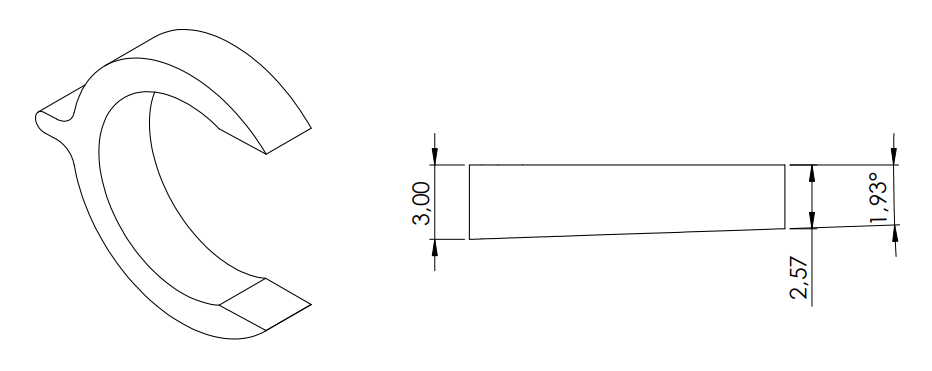
\includegraphics[scale=0.7]{assets/figures/Mechanical Design/MaintientPrism2.png}
    \caption{Prism wedge}
    \label{fig:Prism_Support2}
\end{figure}
The last piece will be used to hold the assembly in position (Figure \ref{fig:Prism_Support3}). It rests on the prism wedges 
and is attached to the support piece (Figure \ref{fig:Prism_Support1}). \newline
During assembly, this part requires particular attention. When tightening the parts, you'll need to tighten each screw a 
little at a time, so that the part remains as parallel as possible to the support.
\begin{figure}[H]
    \centering
    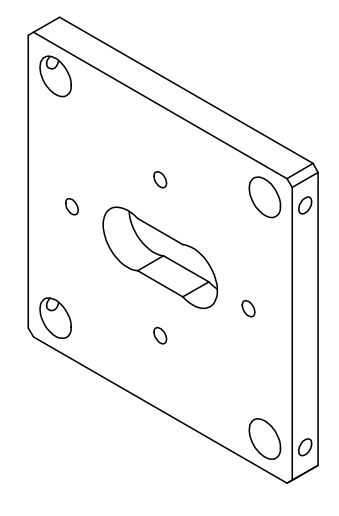
\includegraphics[scale=0.8]{assets/figures/Mechanical Design/MaintientPrism3.png}
    \caption{Clamp for prism support}
    \label{fig:Prism_Support3}
\end{figure}
All these parts will be made of aluminum to reduce its weight. The use of aluminum has no effect on the rigidity of the system.
\bigbreak
The complete drawing can be found in the appendix \ref{App:MEP} for the support and \ref{App:Edmund_MEP} for prisms
%====================================================================================================
% Lens and mounting
%====================================================================================================
\section{Lens and mounting}\label{sec:lens}
\subsection{Lens}
As explained in section \ref{sec:Opti_Limit}, the lens need to be achromatic with a spectrum from 425nm to 675nm 
and a focal lenght of 50mm. For mechanical reasons (size of supports), a 25mm diameter lens had to be integrated. 
\begin{figure}[H]
    \centering
    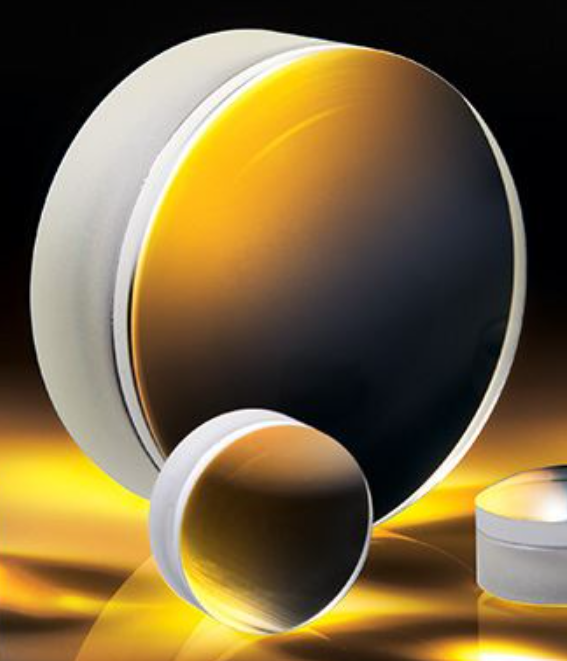
\includegraphics[scale=0.65]{assets/figures/Mechanical Design/Lentille.png}
    \caption{Achromatic lens F = 50mm (425nm - 675nm)}
    \label{fig:Lentille}
\end{figure}
\subsection{Mounting}
This part of the mechanics is much simpler because everything has been ordered from the Edmund optics website. 
The mechanics used to hold the lens in place are a support that attaches to the steel bars, and a cage for 
the lens that attaches directly to the support.
\begin{figure}[H]
    \centering
    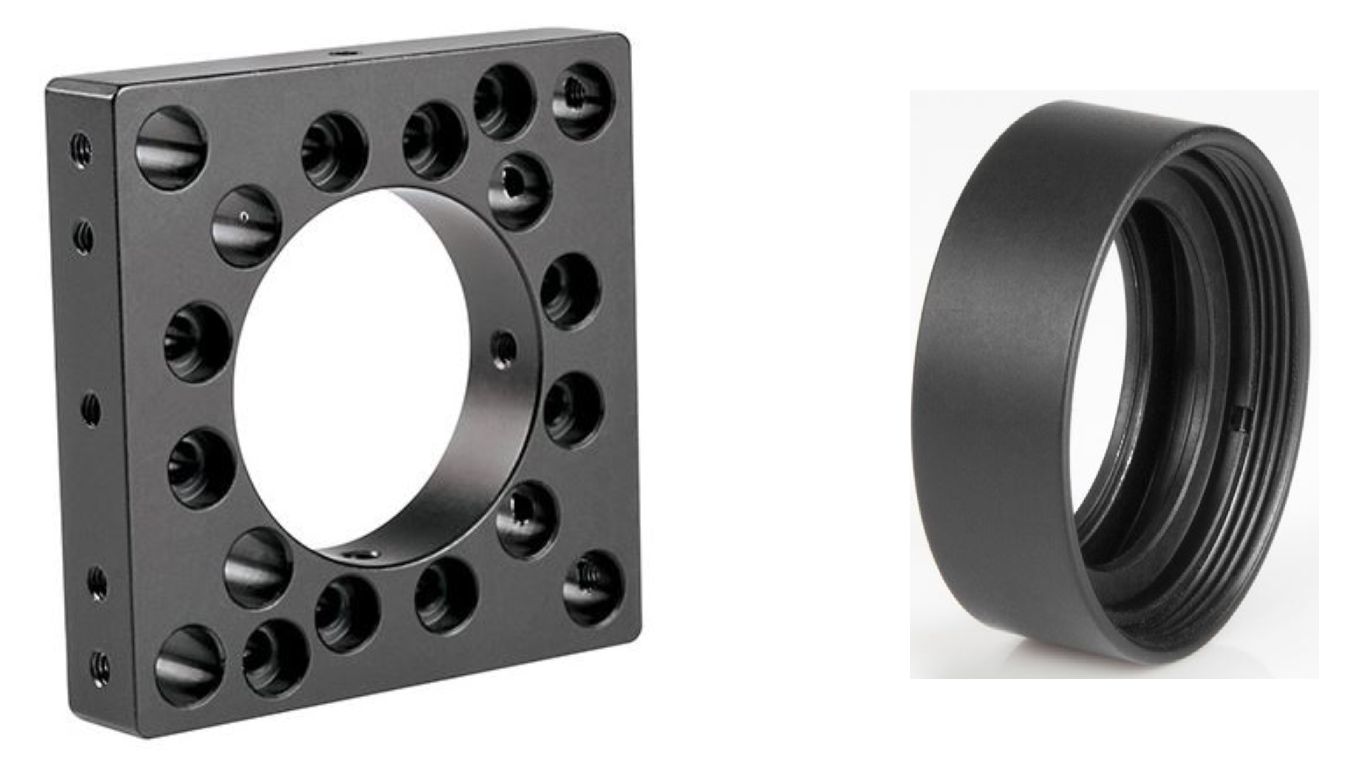
\includegraphics[scale=0.55]{assets/figures/Mechanical Design/Support_Lentille.png}
    \caption{Support and cage for the lens}
    \label{fig:Lentille_Support1}
\end{figure}
\bigbreak
The complete drawing can be found in the appendix \ref{App:Edmund_MEP}
\newpage
%====================================================================================================
% Camera mounting
%====================================================================================================
\section{Camera mounting}\label{sec:Camera}
\subsection{Camera}
As explained in section 2, the chosen camera is Allied Vision's Alvium 1800 U-052m. \newline
It can be mounted on the front panel using either the C-mount thread or four tapped 
holes. It is also possible to attach to these sides with four additional threaded holes.
\begin{figure}[H]
    \centering
    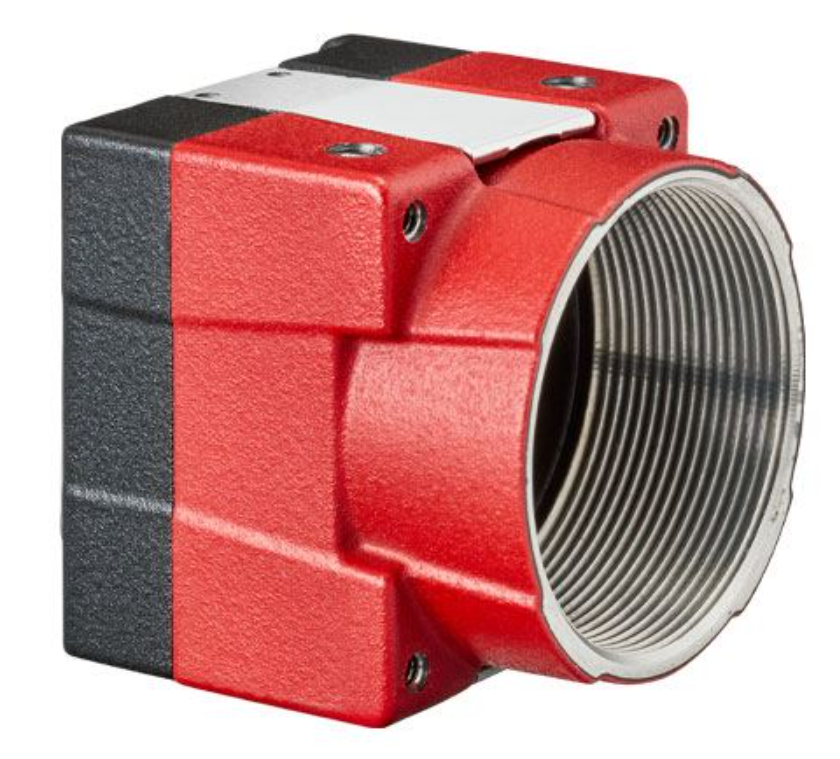
\includegraphics[scale=0.35]{assets/figures/Mechanical Design/Camera.png}
    \caption{Selected camera}
    \label{fig:Camera}
\end{figure}
It was decided to attach the camera via its C-mount thread. After receiving the camera, it was noted that the 
optimum operating temperature for the electronics was 85°C, which causes the casing to heat up considerably. 
It might be necessary to add coolers (or even a fan) at a later date if the tests are not conclusive. 
Other threaded holes could be used to cool the system (cooler attachment).
\subsection{Mounting}
For the camera, a bracket will be designed to hold it in position. The housing has a threading system 
(C-mount) that is very common in the optical world. This is a mounting used for lenses that can be added 
to this type of camera. The part shown in figure \ref{fig:Camera_Support} corresponds to the bracket and comprises 
an external C-mount thread around the shoulder and holes for steel bars.
\break
The camera will be screwed onto the bracket. Its orientation will pose no problem, as the images of our 
stars/sunspots will always be in the sensor area. However, the software will have to be designed to find 
the areas of interest easily and efficiently.
\begin{figure}[H]
    \centering
    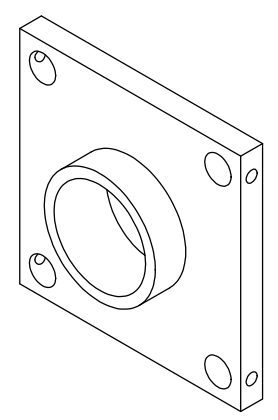
\includegraphics[scale=0.75]{assets/figures/Mechanical Design/Support_Camera.png}
    \caption{Support for the camera}
    \label{fig:Camera_Support}
\end{figure}
\bigbreak
The complete drawing of the support can be found in the appendix \ref{App:MEP} and the drawing of the camera 
in the appendix \ref{App:Edmund_MEP}.